\documentclass[11pt]{article}

\usepackage[a4paper,margin=1in]{geometry}
\usepackage{graphicx}
\usepackage{booktabs}
\usepackage{array}
\usepackage{float}
\usepackage{hyperref}
\usepackage{tabularx}
\usepackage{longtable}
\usepackage{amsmath}
\usepackage{fontspec}
\usepackage{xeCJK}
\usepackage{xcolor}

\setmainfont{TeX Gyre Pagella}
\setCJKmainfont{Noto Serif CJK SC}
\setmonofont{Latin Modern Mono}
\setCJKmonofont{Noto Sans Mono CJK SC}
\linespread{1.08}
\hypersetup{colorlinks=true,linkcolor=blue,urlcolor=blue}

\title{Where Hidden Rhythms in Silent Vectors Lie:\\
Character-Level GPT for Chinese Poetry}
\author{}
\date{April 9, 2026}

\begin{document}
\maketitle

\begin{abstract}
This report presents a character-level decoder-only Transformer trained on a 5 MB corpus of Chinese \emph{Song ci}. The goal was not only to obtain a working text generator, but also to study how poetic structure emerges during training and inside the model's internal representations. I implemented a multi-head causal decoder in PyTorch, compared the SDPA attention backend against a classic masked-attention implementation, trained a main baseline on an RTX 3090 Ti, explored three hyperparameter variations, analysed generated poems against corpus statistics, and ran a probing experiment on newline prediction. The main findings are that (i) SDPA is clearly preferable in both speed and memory, (ii) a 6-layer, 256-dimensional model with context length 256 learns convincing line-level poetic structure, (iii) validation performance peaks around 6k steps and then degrades with further training, (iv) shorter context and shallower depth both hurt validation loss, and (v) hidden states of the trained model encode line-boundary information much more strongly than those of a random model with the same architecture.
\end{abstract}

\section{Introduction}
The assignment asked for a character-level GPT-like model trained on poetry, with explicit monitoring of training and at least one analysis of internal structure. I chose this framing as a compact but meaningful test-bed for studying emergence: character-level modelling keeps the vocabulary small and the implementation manageable, while poetry preserves visible structure such as line length, line boundaries, punctuation, and recurrent imagery.

The lab was organised around four questions:
\begin{enumerate}
    \item Can a small decoder-only Transformer learn to generate plausible Chinese poetic continuations?
    \item Which implementation choices matter most for efficient training?
    \item How do context length, depth, and dropout affect behaviour?
    \item Do the hidden states encode an interpretable structural signal, namely the presence of an upcoming newline?
\end{enumerate}

\section{Corpus and Data Pipeline}
The main corpus is \texttt{songci\_main\_5mb.txt}, derived from a larger Chinese poetry repository. Song \emph{ci} was chosen because it offers a useful compromise between lexical richness and strong visible form. Line breaks, stanza boundaries, and punctuation were preserved exactly, as required by the assignment.

Corpus-level statistics for the main training file are:
\begin{itemize}
    \item 20{,}773 poems
    \item 157{,}179 lines
    \item average 7.57 lines per poem
    \item average raw line length 10.74 characters
    \item average line length after punctuation removal 8.91 characters
\end{itemize}

The model operates strictly at character level. I constructed a sorted character vocabulary directly from the corpus, obtaining a vocabulary size of 6{,}080 characters in the main run. The text was encoded as integer IDs, split into 90\% training and 10\% validation, and sampled into random fixed-length contexts during training.

This choice keeps the pipeline simple and avoids tokenisation confounds. It also makes probing easier because boundaries such as \texttt{\textbackslash n} are explicit characters rather than latent tokenisation artefacts.

\section{Model and Implementation Choices}
The final implementation is a decoder-only Transformer with:
\begin{itemize}
    \item learned token embeddings
    \item learned positional embeddings
    \item pre-norm residual blocks
    \item multi-head causal self-attention
    \item 4$\times$ expansion feed-forward networks with GELU
    \item a final LayerNorm and linear vocabulary projection
\end{itemize}

The baseline configuration follows the assignment closely:
\begin{itemize}
    \item context length 256
    \item 6 layers
    \item hidden size 256
    \item 8 heads
    \item batch size 32
    \item AdamW with learning rate $3 \times 10^{-4}$
    \item dropout 0.1
    \item 500 warm-up steps
\end{itemize}

I implemented two attention backends:
\begin{enumerate}
    \item \texttt{torch.nn.functional.scaled\_dot\_product\_attention} (\texttt{sdpa})
    \item a classic masked-attention implementation using an explicit causal mask
\end{enumerate}

The benchmark in Figure~\ref{fig:benchmark} shows that \texttt{sdpa} is clearly superior on the target configuration. On GPU, \texttt{sdpa} required only 2.172 ms per step and 114 MB peak memory, versus 3.858 ms and 331 MB for the classic implementation. This is a large enough gap that \texttt{sdpa} is the only reasonable choice for the main experiments.

\begin{figure}[H]
    \centering
    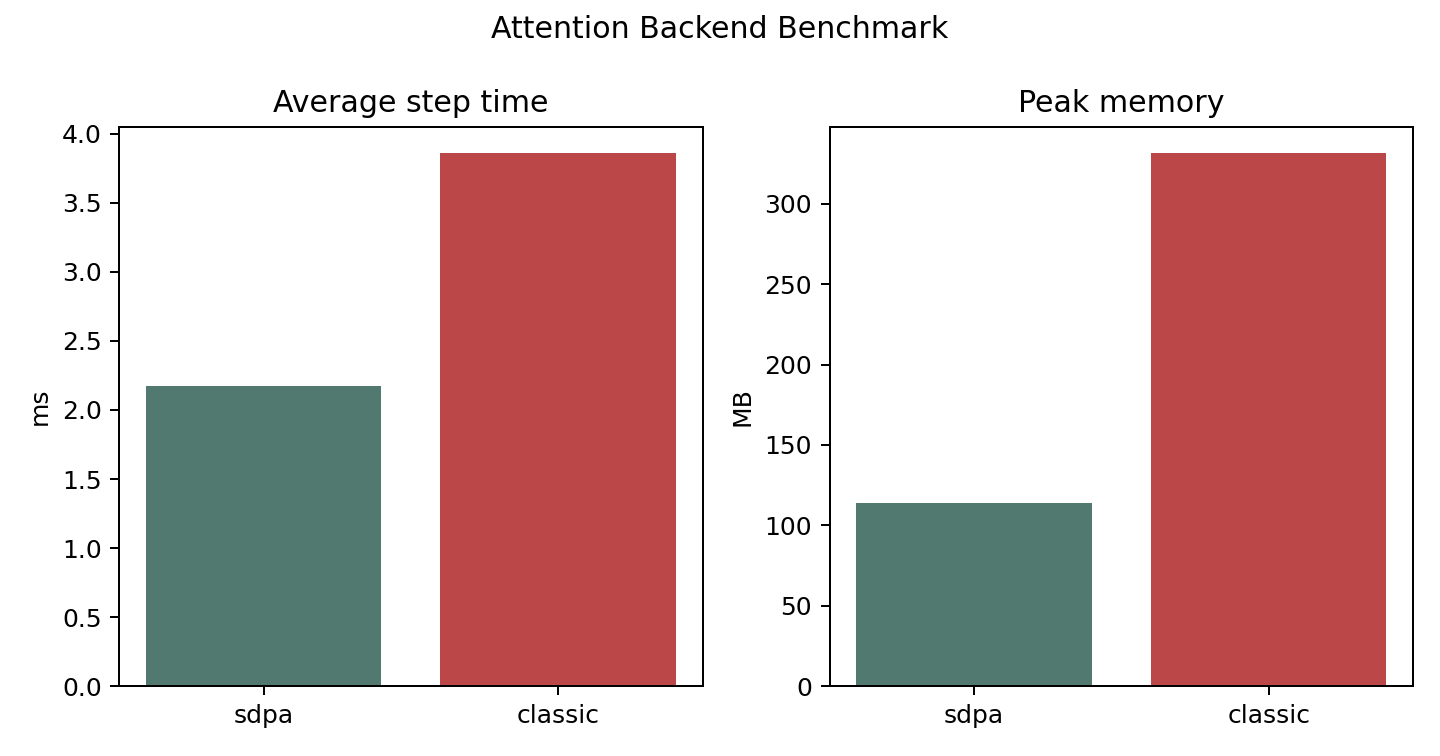
\includegraphics[width=0.82\linewidth]{report_assets/attention_benchmark.png}
    \caption{Attention backend benchmark on the RTX 3090 Ti. \texttt{sdpa} is both faster and much more memory-efficient than classic masked attention.}
    \label{fig:benchmark}
\end{figure}

\section{Training and Monitoring}
The main long run used the baseline architecture on \texttt{songci\_main\_5mb.txt} for 20k steps. During training I logged train loss, validation loss, bits-per-character (BPC), generated samples, and checkpoints. The most important outcome is shown in Figure~\ref{fig:training}.

\begin{figure}[H]
    \centering
    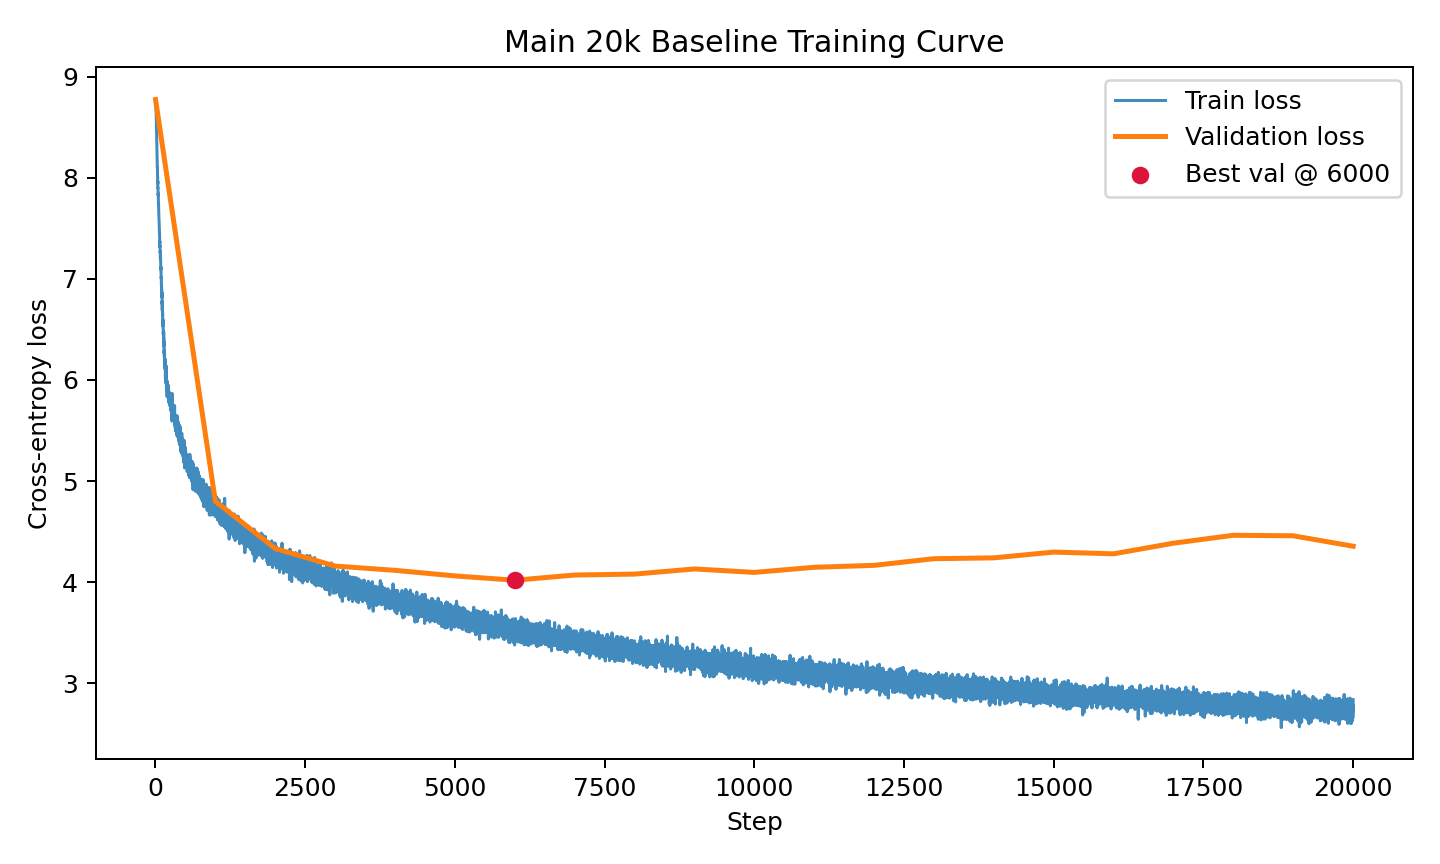
\includegraphics[width=0.84\linewidth]{report_assets/training_curve_20k.png}
    \caption{Training and validation loss for the 20k-step baseline. Validation improves quickly, reaches its best value near 6k steps, and then gradually worsens while train loss continues to decrease.}
    \label{fig:training}
\end{figure}

The 20k run produced the following key results:
\begin{itemize}
    \item final train loss: 2.8377
    \item final validation loss: 4.3550
    \item best validation loss: 4.0186 at step 6000
    \item final validation BPC: 6.2829
\end{itemize}

This is an important result in itself. The model clearly learns, but more training is not monotonically better. Validation loss decreases up to around 6k steps, then rises again. This means the run enters an overfitting regime after the best checkpoint region. In practice, the correct conclusion is not ``train as long as possible'', but rather ``train long enough to identify the best checkpoint and stop there''.

This is also why I used the saved 5k checkpoint for the qualitative and structural analyses below: it lies near the best-performing region, while the 20k final checkpoint is already overtrained.

\section{Hyperparameter Exploration}
To keep the comparison controlled, I varied one parameter at a time for 2k-step runs under the same optimiser and batch-size settings. The compared settings were:
\begin{itemize}
    \item context length 128 instead of 256
    \item 4 layers instead of 6
    \item dropout 0.0 instead of 0.1
\end{itemize}

The summary appears in Figure~\ref{fig:hparams} and Table~\ref{tab:hparams}.

\begin{figure}[H]
    \centering
    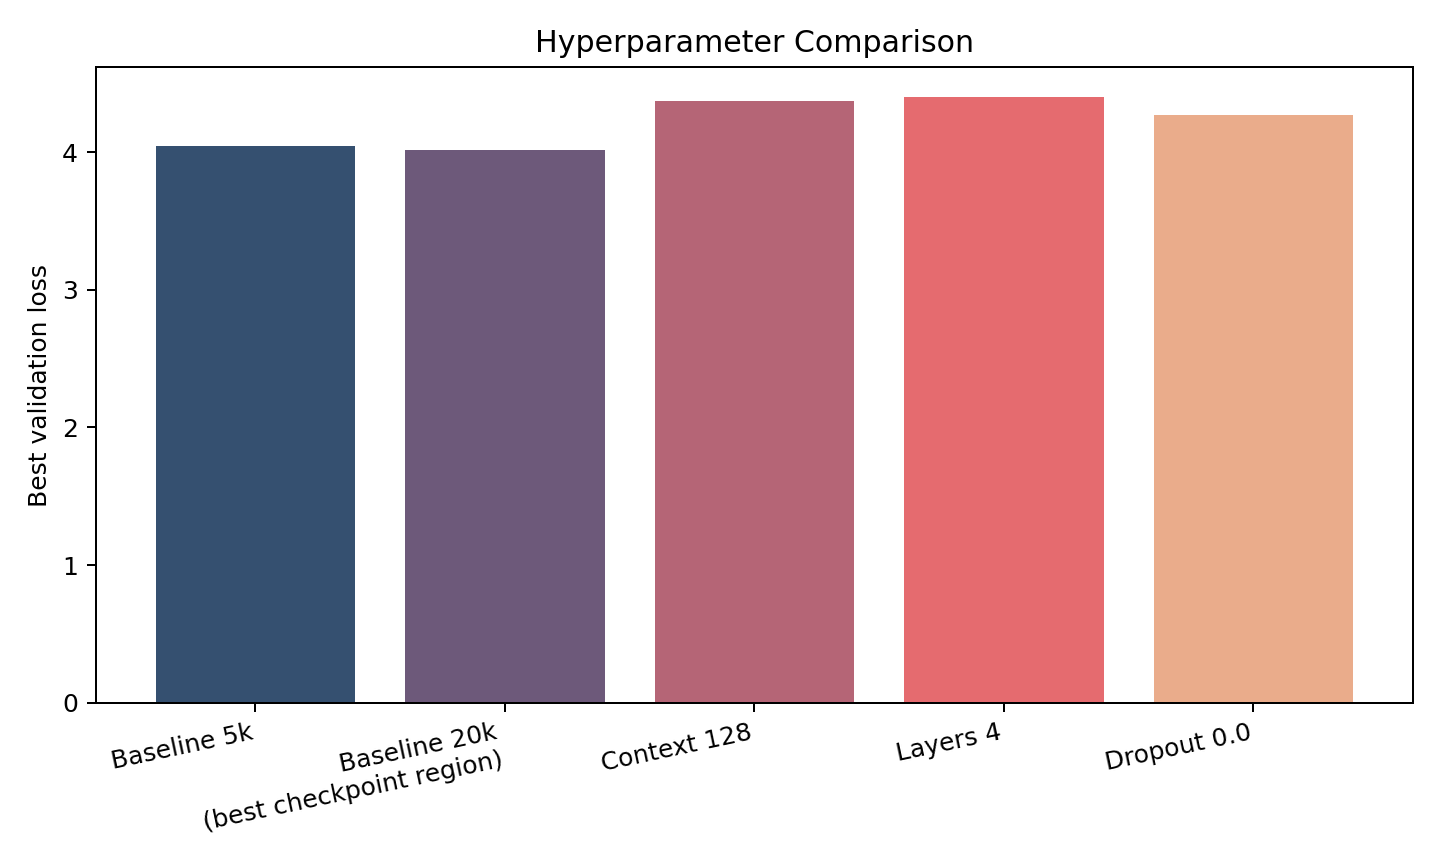
\includegraphics[width=0.82\linewidth]{report_assets/hyperparameter_comparison.png}
    \caption{Best validation loss for the main runs and the three controlled hyperparameter variants. Lower is better.}
    \label{fig:hparams}
\end{figure}

\begin{table}[H]
    \centering
    \small
    \begin{tabular}{lccc}
        \toprule
        Run & Steps & Best Val Loss & Main Interpretation \\
        \midrule
        Baseline 20k & 20{,}000 & 4.0186 & Best region near step 6000 \\
        Baseline 5k & 5{,}000 & 4.0411 & Strong saved checkpoint near optimum \\
        Context 128 & 2{,}000 & 4.3677 & Worse than context 256 \\
        Layers 4 & 2{,}000 & 4.3967 & Worse than 6 layers \\
        Dropout 0.0 & 2{,}000 & 4.2696 & Better early optimisation than 0.1 \\
        \bottomrule
    \end{tabular}
    \caption{Controlled hyperparameter study.}
    \label{tab:hparams}
\end{table}

These experiments support three concrete claims.

\paragraph{Context length matters.}
The 128-context model is clearly worse than the 256-context baseline. This supports the assignment's suggestion that 256 is a more appropriate length for capturing inter-line dependencies and larger poetic units.

\paragraph{Depth matters.}
Reducing the model from 6 layers to 4 layers also hurts validation loss. The 4-layer model trains faster, but it sacrifices modelling power. This is a meaningful trade-off: lower compute, weaker performance.

\paragraph{Dropout interacts with training horizon.}
At 2k steps, removing dropout improved validation loss relative to the short 0.1-dropout runs. My interpretation is that, for this corpus and this early-training window, dropout 0.1 slightly slows optimisation. However, the long 20k run also shows that overfitting is real, so I would not conclude that dropout should always be zero. The correct interpretation is more cautious: dropout affects the speed--regularisation trade-off, and the preferred value depends on training duration and checkpoint selection.

\section{Analysis of Generated Poems}
For qualitative analysis, I generated 100 continuations from the 5k checkpoint using temperature 0.85 and top-$k$ sampling with $k=20$. Two representative outputs are shown below.

\paragraph{Generated poem A.}
\begin{quote}\small
君不见，不如飞。\\
何处西湖，江南岸月，几番风雨。\\
\\
记得春归，故园曾到东篱。\\
小桥烟草，几重来、清香浮动，犹恋寒梢。\\
东篱菊蕊，依然还是，玉楼十二，雪花空。\\
谁知道，何逊扬州。\\
想桃花好，花上一枝春。\\
想香心，香凝雪后，有人知。\\
天公此意，何须更有，有山翁、不是人间。
\end{quote}

\paragraph{Generated poem B.}
\begin{quote}\small
一番秋色。\\
不是秋光消瘦影。\\
人与孤标，一枝不比孤芳意。\\
小窗斜影朦胧影。\\
夜半残更漏残更。\\
\\
梦云飞、一掬清秋色。\\
梦入东窗，半窗风竹。\\
\\
花影横斜，柳阴满地红湿。\\
芳意渐远，花飞不尽，愁难觅。\\
玉箫人去空留客。\\
又唤起、西风吹笛。
\end{quote}

These samples are not fully coherent poems, but they are already much more than random text. The model produces line breaks, punctuation, recurrent motifs (\emph{wind}, \emph{flowers}, \emph{spring}, \emph{autumn}, \emph{jade}, \emph{moon}), and a recognisable register close to the training corpus. The main failure modes are lexical repetition, weak global planning, and unstable poem length.

To quantify this, I compared the generated corpus against the reference corpus. Figure~\ref{fig:structure} shows the raw line-length distribution.

\begin{figure}[H]
    \centering
    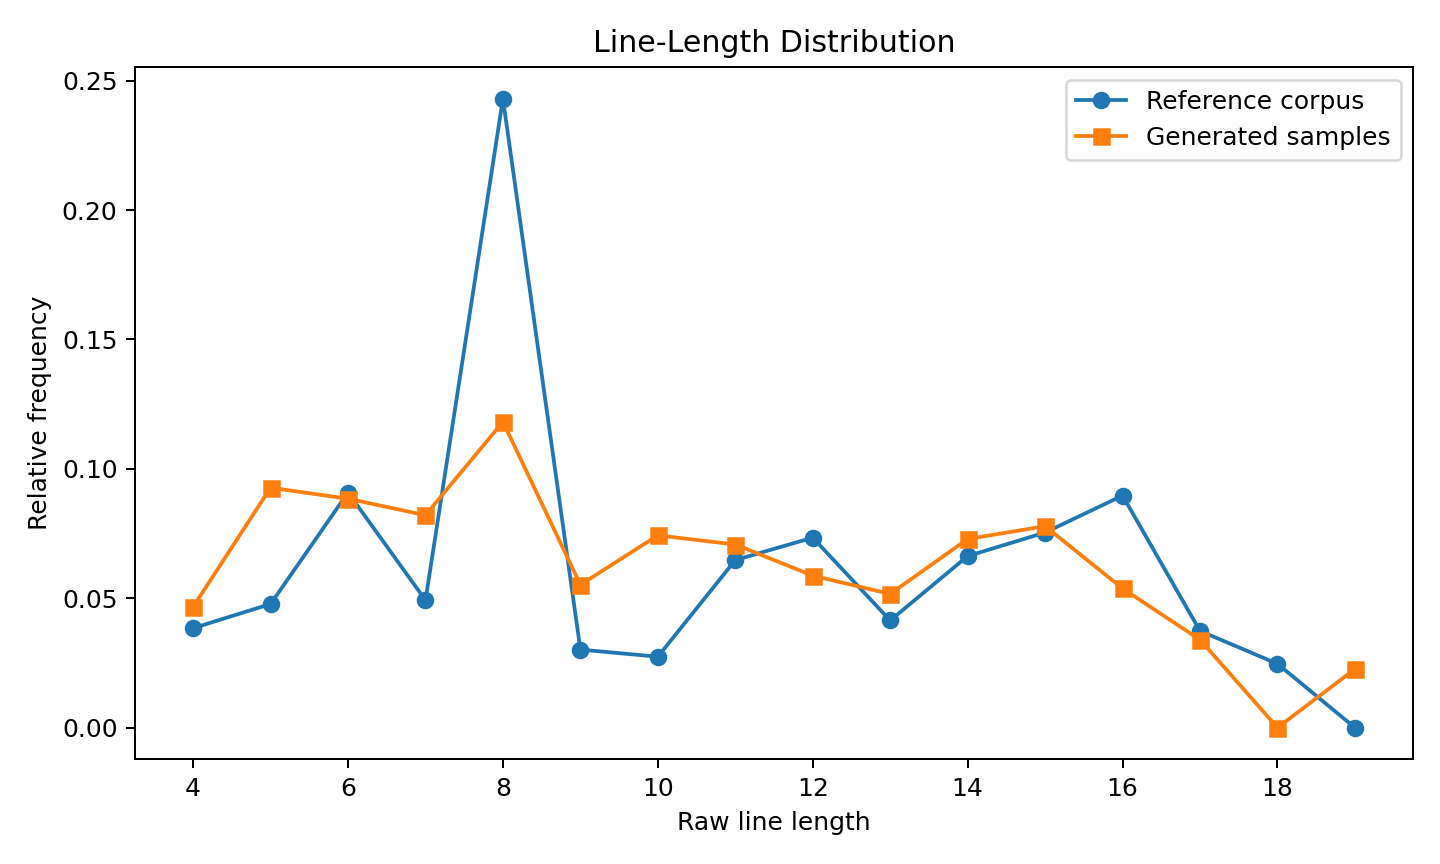
\includegraphics[width=0.84\linewidth]{report_assets/structure_line_lengths.png}
    \caption{Reference versus generated raw line-length distributions. The match is reasonably close, which suggests that local line-level form is learned well.}
    \label{fig:structure}
\end{figure}

The main structural comparison gave the following results:
\begin{itemize}
    \item reference average raw line length: 10.74
    \item generated average raw line length: 10.50
    \item reference average stripped line length: 8.91
    \item generated average stripped line length: 8.58
    \item reference punctuation ratio: 0.1706
    \item generated punctuation ratio: 0.1828
    \item line-ending distribution L1 gap: 0.1065
\end{itemize}

These numbers show that local structure is captured surprisingly well. Line length and punctuation density are close to the corpus. The major failure lies elsewhere: the generated samples average 15.4 lines per poem, whereas the reference corpus averages only 7.57. In other words, the model has learned how lines look, but not yet how long a poem should be.

\section{Probing Internal Representations}
The final experiment asks whether internal states encode a structural signal. I tested this with a simple linear probe: given the final hidden state at each position, can a linear classifier predict whether the \emph{next} character is a newline?

The probe was trained on frozen hidden states from the 5k checkpoint and compared against a random model with the same architecture. Results appear in Figure~\ref{fig:probe}.

\begin{figure}[H]
    \centering
    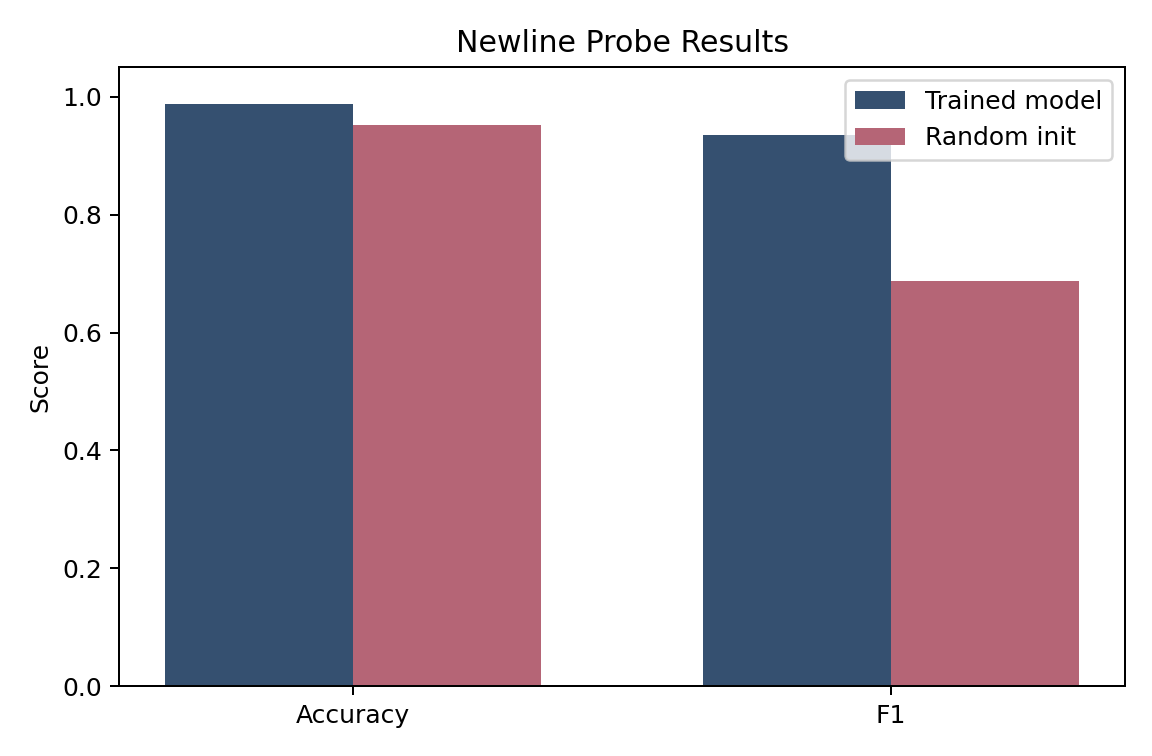
\includegraphics[width=0.72\linewidth]{report_assets/probe_newline.png}
    \caption{Linear probe performance for predicting whether the next character is a newline. The trained model substantially outperforms the random baseline.}
    \label{fig:probe}
\end{figure}

Quantitatively:
\begin{itemize}
    \item trained-model accuracy: 0.9880
    \item trained-model F1: 0.9343
    \item random-initialised-model accuracy: 0.9517
    \item random-initialised-model F1: 0.6882
    \item F1 gain: +0.2461
\end{itemize}

This is a strong result. Even a random model can capture some boundary signal because the task is imbalanced and hidden states still carry local information from the input itself. But the trained model does much better, especially in recall and F1. This means that newline structure is encoded much more explicitly after training. In the terms of the assignment, this is direct evidence that an interpretable structural property emerges inside the model's representations.

\section{Discussion}
The most important lesson from these experiments is that different levels of poetic structure emerge at different rates.

At the local level, the model learns quickly. By a few thousand steps it already captures line length, punctuation, and common lexical fields. This is visible both qualitatively and in the structural statistics.

At the global level, the model remains weaker. It overproduces lines, repeats motifs, and often drifts into self-reinforcing continuations. This is consistent with the fact that global poem planning is a harder task than modelling local line continuation.

The hyperparameter study reinforces this interpretation. Shorter context and shallower depth both degrade performance, which suggests that wider receptive field and more hierarchical computation help the model organise line-level and cross-line structure. At the same time, the long 20k run shows that more optimisation is not sufficient by itself: once validation begins to rise, the model increasingly specialises to the training distribution in a less general way.

The probe result complements the generation results. It shows that line-boundary information is not only present in the output, but also linearly recoverable from internal hidden states. This is exactly the kind of emergence the lab was designed to study.

\section{Conclusion}
This project succeeded on both fronts required by the lab: building a working character-level GPT-style poetry generator and investigating the emergence of structure inside the model.

The final conclusions are:
\begin{itemize}
    \item \texttt{sdpa} is the correct attention backend for this project because it is both faster and more memory-efficient.
    \item A 6-layer, 256-dimensional decoder with context length 256 learns convincing local poetic structure on a 5 MB Song \emph{ci} corpus.
    \item Validation performance peaks around 6k steps, so checkpoint selection matters more than simply training longer.
    \item Longer context and greater depth are both useful, while dropout trades off early optimisation against regularisation.
    \item The trained model's hidden states encode newline structure much more strongly than those of a random baseline.
\end{itemize}

The main limitation is that global poem-level control is still weak. If I continued this project, I would first save checkpoints more frequently around the best-validation region, then compare Song \emph{ci} against the Tang regulated-verse subset, and finally add a richer probing setup beyond newline prediction, for example line-position or punctuation prediction.

\end{document}
